\begin{itemize}
    \item Zusammenfassung der Resultate
    \item Hier geben Sie wieder, was aus der Arbeit als Ergebnis resultiert. Es ist darauf zu achten, dass keine Bewertung der Daten vorweggenommen wird. Diese soll im Diskussionsteil erfolgen. Trotzdem sind die Daten und Resultate mit genügend Text zu erklären. Absolut zentral ist dabei eine präzise, treffende sprachliche Ausdrucksweise. Von Alltagsslang und vagen Ausdrücken ist unbedingt abzusehen.
          Bei grossen Datenmengen müssen die Rohdaten nicht zwingend publiziert werden.
\end{itemize}

This chapter provides the result of the different approaches that have been used during the evaluation phase. Starting off the exploration algorithm tests were made based on visual tests of the Python plots. Then the test results of the optimization algorithm will be presented along with the different output of the program. To round up the integration tests are presented with the test on the simulation tool.

\section{Exploration Algorithm}
The exploration algorithm test were made via the python plots. CSV files were used from the \acrlong{tum} to have track information like the position of the cones and the car in an abstract data format. \cite{tumftm_optimization_algoritm} Figure \ref{fig:Result acceleration} shows the first approach (top left image), the second (top right image) and the final approach (bottom image) side by side on the acceleration track which was mentioned in section \ref{sec:Dynamic Events}. Since the plot on the top left and right side does not plot the start cones and the end cones in orange it was just used as a basis for the final more usable algorithm implementation (bottom image). The second approach calculated middle points between the grouped 4 points that where used for the triangulation. In addition to the added points a line was drawn to smoothen the track.

\begin{figure}[H]
    \centering
    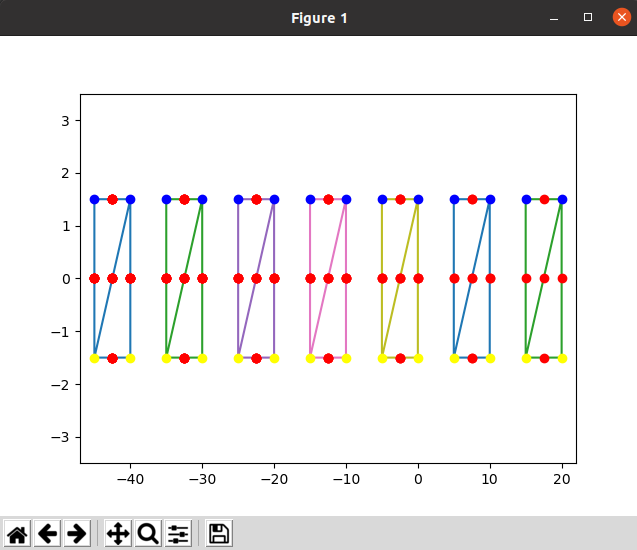
\includegraphics[width=6.5cm]{Result_First_Delauney_Acceleration.png}\hfill
    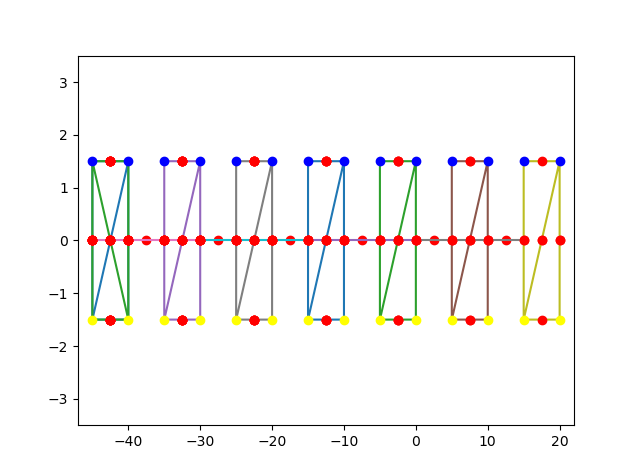
\includegraphics[width=6.5cm]{Result_First_Middle_Point_Acceleration.png}
    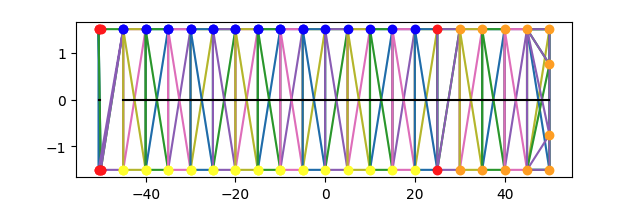
\includegraphics[width=6.5cm]{Result_Acceleration_final.png}
    \caption{The image on the top left shows the first approach on the acceleration track and the image on the top right the second, while drawing a middle line. The image on the bottom shows the final approach.}
    \label{fig:Result acceleration}
\end{figure}

The second track that was used for comparison is one of the \acrlong{tum} team which is called ``Small Track''. \cite{tumftm_optimization_algoritm} This track helped to get an understanding how the algorithm works on corners with fewer cones on the inner side then on the outer side. Figure \ref{fig:Result small track} shows a progression of the improvements of the first implementation of the algorithm (top left image) to the second improved version (top right image) and the final version of the algorithm (bottom image). Again for the first and the second approach the implementation of publishing orange cones was not made already.

\begin{figure}[H]
    \centering
    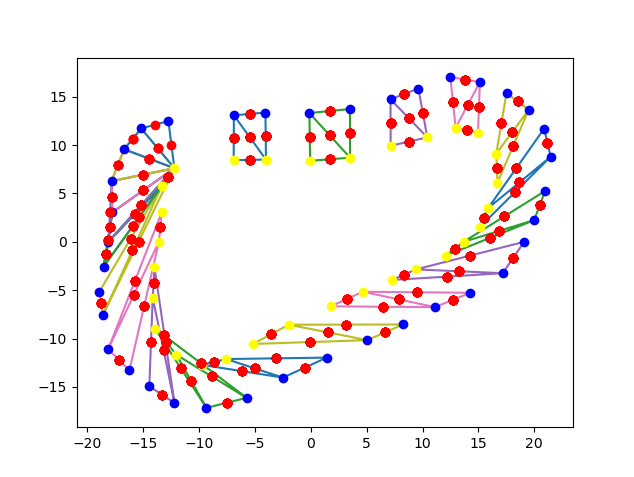
\includegraphics[width=6.5cm]{Result_First_Delauney.png}\hfill
    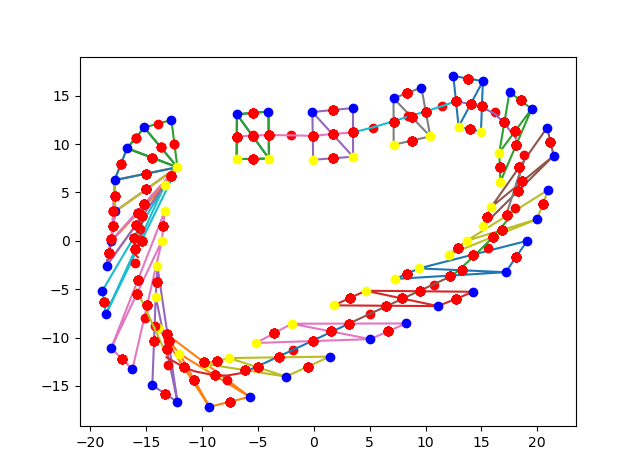
\includegraphics[width=6.5cm]{Result_First_Middle_Line_Approach.png}
    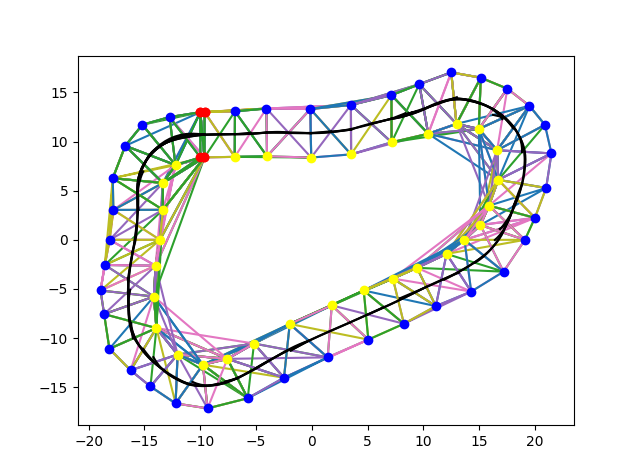
\includegraphics[width=6.5cm]{Result_SmallTrack_final.png}
    \caption{Progression of the improvement of the first implementation (top left image) to the second (top right image) and to the final implementation (bottom image).}
    \label{fig:Result small track}
\end{figure}

The next track which is showed in figure \ref{fig:Result final middle line rand track} that was used for testing the final implementation was the ``Rand'' track. It has more cones and curvature compared to the ``Small Track'' and shows an example of a track that could have been used for the third track in the competition. As described in the competition rules the track properties of ``Acceleration'' and ``Skidpad'' where given already. More information can be found in section \ref{sec:Dynamic Events}.
\begin{figure}[H]
    \centering
    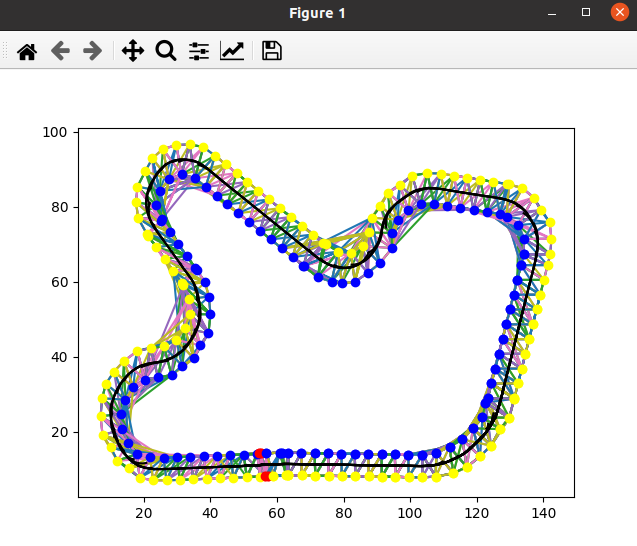
\includegraphics[width=7cm]{Result_Rand_Triangulation_final.png}
    \caption{The ``Rand'' track with the final algorithm implementation}
    \label{fig:Result final middle line rand track}
\end{figure}

Furthermore, a track which was used for the competition of 2021 is shown in figure \ref{fig:Result final middle line 2021 competition track} with the applied final exploration algorithm. The track consists of more corners than the ``Rand'' track.
\begin{figure}[H]
    \centering
    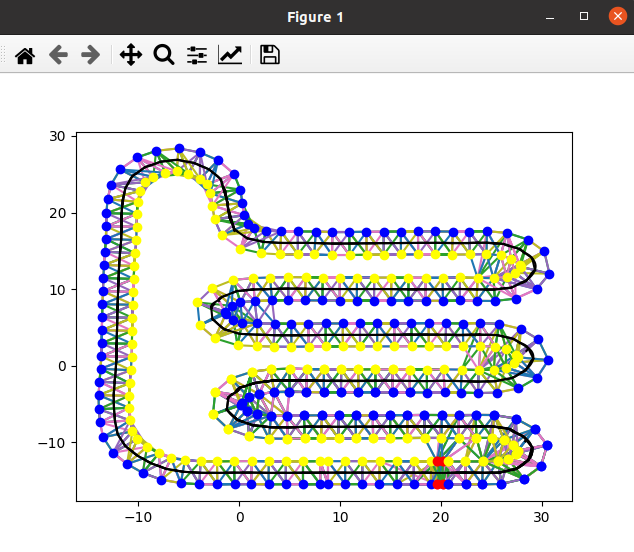
\includegraphics[width=7cm]{Result_Comp2021_middle_line_final.png}
    \caption{The result of the final exploration algorithm applied on the competition track of 2021.}
    \label{fig:Result final middle line 2021 competition track}
\end{figure}

The last example in figure \ref{fig:Result final middle line skidpad track} shows that the algorithm can be applied on the ``Skidpad'' track.
\begin{figure}[H]
    \centering
    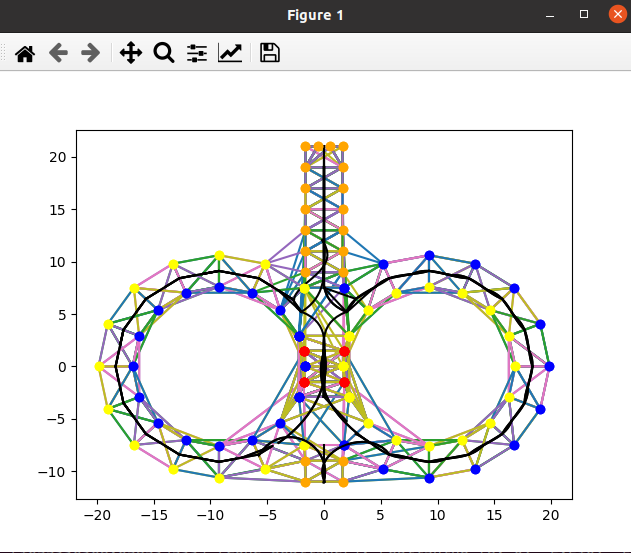
\includegraphics[width=7cm]{Result_Skidpad_final.png}
    \caption{The first try to calculate the middle line with the }
    \label{fig:Result final middle line skidpad track}
\end{figure}

\section{Optimization Algorithm}
\begin{itemize}
    \item verschiedene Screenshot
    \item Zeiten auswertung / vergleich / übersicht
\end{itemize}
Optimization times for berlin\_2018

shortest\_path = 16.72s
Estimated lap time: 89.12s

mincurv = 44.40s
Estimated lap time: 82.46s

mincurv\_iqp = 127.69s
Estimated lap time: 81.06s

mintime = 92.00s
Estimated lap time: 85.77s

\section{Integration}
\begin{itemize}
    \item Test im Python Plots
    \item Simulationstool (Screenshot, evtl. folge von Screenshots), welche strecke (grafik simulationstool)
\end{itemize}

